\chapter{Experiment Data and Analysis}

\section{Overview of The Balloon Experiments}

High altitude balloons have an extensive heritage as platforms for experiments that take place in the upper atmosphere. In this chapter we will examine results from three balloon flight campaigns which carried X-ray spectrometers. The results of the previous two chapters will be applied to determine as much information about the causative precipitating electrons as possible, while avoiding over-fitting the available data. The total precipitating flux and energy distribution of the electrons will be the main targets. The experiments on the balloon flights that we use in this chapter were all equipped with NaI scintillator detectors, and the analysis will be framed around the data that can be obtained from them. There will be questions that can be answered using detectors of a different design, particularly, those sensitive to the angular distribution of the incoming photons. These will be discussed at the end and left for future work. 

The balloon flights used in this analysis were from the following campaigns.

\begin{center}
\begin{tabular}{ |c|c|c|c| } 
\hline
Project Name & Location & Active & Primary Reference \\
\hline
$\text{ABOVE}^2$ & Saskatoon, Saskatchewan & Summer 2016 & None Current\\
\hline
BARREL & Antarctica & 2013-2014 & \citet{Millan2014}\\
\hline
EPEX & Fort MacMurray, Alberta & Summer 2018 & None Current\\
\hline
\end{tabular}
\end{center}

The campaigns each consisted of a number of flights. Each had a somewhat different scientific target, which will be discussed in their analysis sections, however, all of them carried NaI scintillation detectors of a similar design, which we can use with the results from the previous two chapters. We will begin with a discussion of the detector design and operating principles. 

\section{Detector Design}

The sodium iodide scintillation detector carried by flights on all three balloon campaigns was designed by Dr. Michael McCarthy at the University of Washington, Seattle campus. The instrument design has a heritage extending back to~\citet{winckler}. The instrument specifications follow, reproduced from~\citet{Millan2014}. 

\begin{center}
\begin{tabular}{ |c|c|c|c|c| }
\hline
Attribute & Value & Comments \\
\hline
Mass & 2.8 Kg & includes insulation and harness \\
Energy Range & 20 keV to 10 MeV & \\
Electronics Resolution & 2.4 keV / channel & reduced by binning \\
System Resolution & 7 percent at 662 keV & \\
Effective Area & 16$\text{ cm}^2$ at 1 MeV & \\
Dead time Per Event & 52 $\mu\text{s}$ & \\
Operating Temperature & -10 to 40 deg C & efficiency decreases below 15 deg C \\
Voltage Requirement & +/- 5 V DC & \\
Current Requirement & 40 mA +, 10 mA - & depends on count rate\\
\hline
\end{tabular}
\end{center}

Simulations completed with GEANT3 (the predecessor to GEANT4) indicate that the detector behaves as essentially uncollimated, though the view through the atmosphere results in it having a field of view of approximately 60 degrees~\citet{Millan2014}. 

A picture of the detector as flown on the $\text{ABOVE}^2$ campaign is shown in Figure~\ref{detector_picture}. The unit is cylindrical, standing on a plexiglass mount and standing approximately 30 cm tall. The cylinder includes the NaI scintillation crystal, photomultiplier tube, and optical coupling. X-rays deposit their energy in the NaI crystal, and a fraction of the resulting light pulse is converted to a voltage pulse by the photomultiplier tube~\citet{Millan2014}. This voltage pulse is then converted to a digital value proportional to the deposited energy by the DPU and output on a serial port for processing and storage by the rest of the flight system. The disconnected wire harnesses visible in Figure~\ref{detector_picture} connect the detector to the various support hardware included with the flight system. Temperature sensors and heaters were used to maintain the detector temperature at 15 deg. C during the flight. Power was provided by an array of lithium-ion rechargeable batteries, which are contained in the rectangular foam box behind the detector in Figure~\ref{detector_picture}.

\begin{figure}[p]
    \centering
    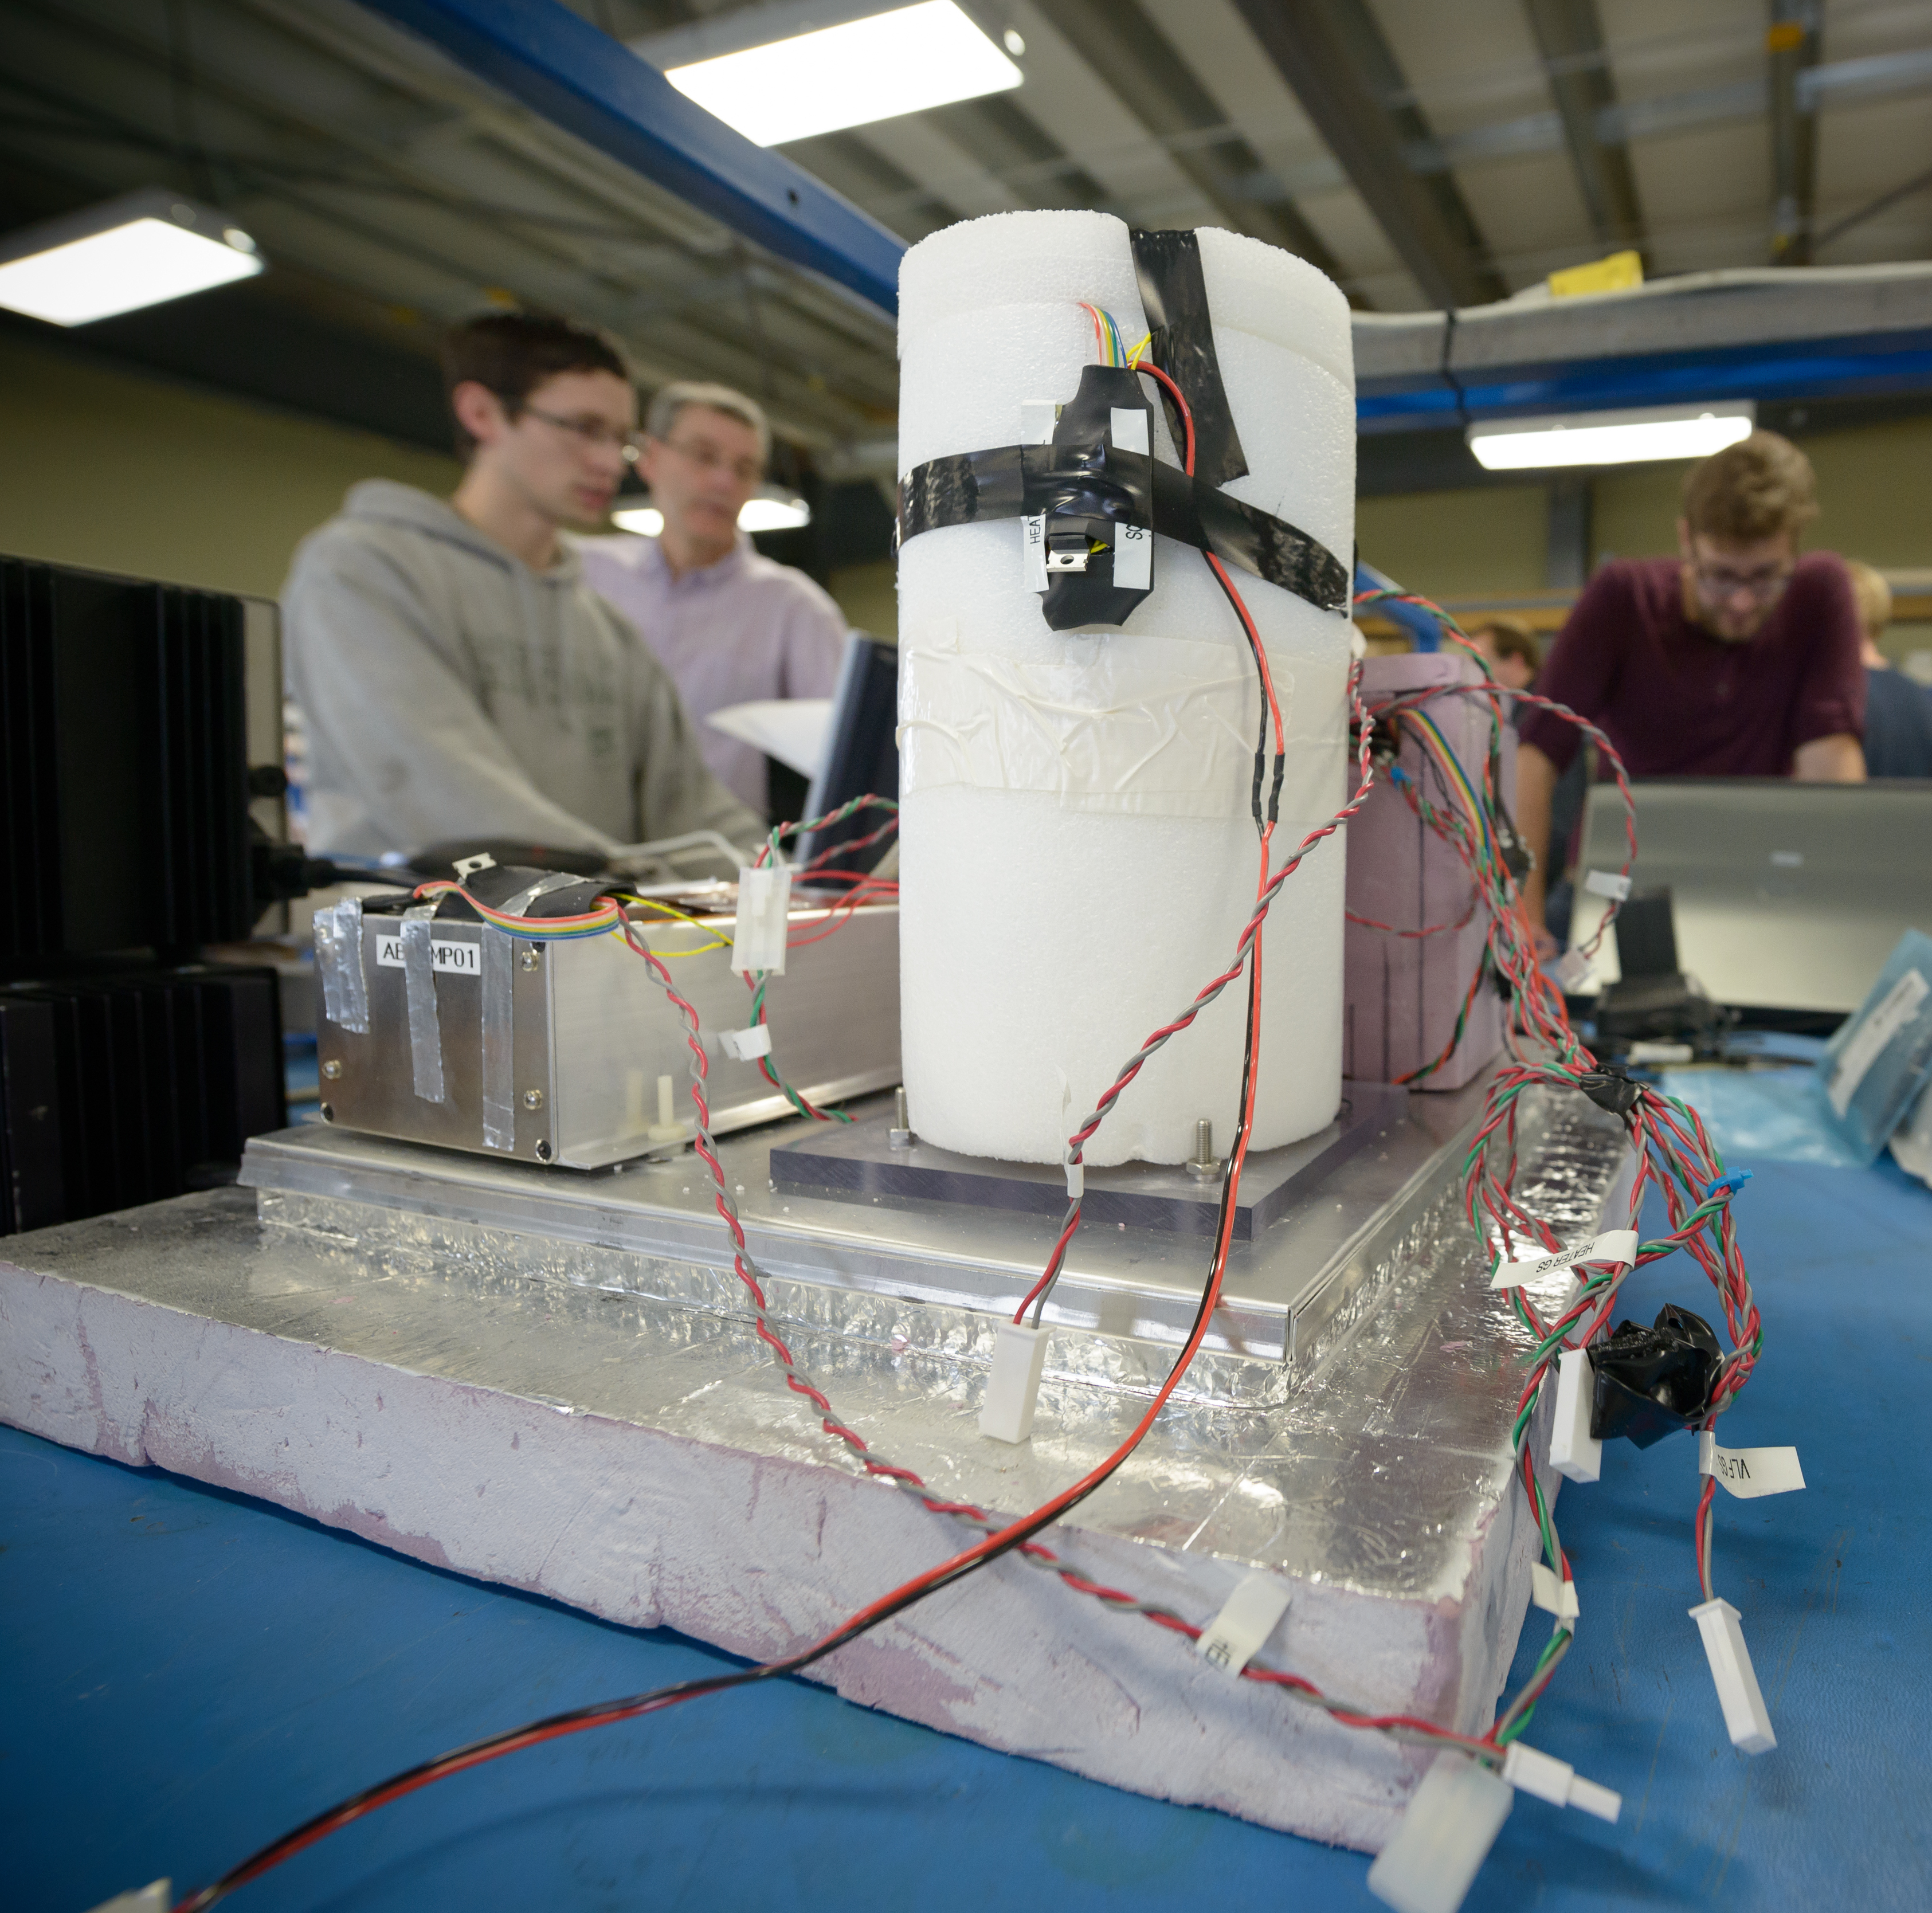
\includegraphics[width=1.0\textwidth]{figures/chapter_5/detector_picture/detector_picture.jpg}
    \caption{X-ray spectrometer (white cylinder) encased in insulation foam and installed with flight systems in balloon payload. The DPU (digital processing unit) is contained in the metal rectangular enclosure on the left. The lead collimator assembly has been removed from the detector during testing.}
    \label{detector_picture}
\end{figure}

The detector sends measurements to a serial port as digital data. The outputs, reproduced from~\citet{Millan2014}, follow.

\begin{center}
\begin{tabular}{ |c|c|c|c|c| }
\hline
Product & Cadence & Energy Range (keV) & No. of Energy Channels \\
\hline
Rate Counters & 4 & - & - \\
Fast Spectra & 0.05 & 20-1500 & 4 \\
Medium Spectra & 4 & 100-4000 & 48 \\
Slow Spectra & 32 & 20-10000 & 256 \\
\hline
\end{tabular}
\end{center}

For the EPEX and $\text{ABOVE}^2$ campaigns, the instruments were designed to be recovered, and the data were recorded to onboard storage, with some telemetered results as a backup. For the BARREL campaign, the logistics involved in recovering all the payloads are difficult. While a subset were recovered, most were not, and the data were telemetered using an iridium satellite modem. For these flights, the analysis uses the data products published at NASA CDAWEB. The primary citation for this data set is~\citet{Millan2014}.

The functional layout of the detector is shown in the block diagram of Figure~\ref{detector_block_diagram}, which is reproduced from~\citet{Millan2014}.

\begin{figure}[p]
    \centering
    \includegraphics[width=1.0\textwidth]{figures/chapter_5/detector_block_diagram/detector_block_diagram}
    \caption{Block diagram of X-ray scintillation detector system}
    \label{detector_block_diagram}
\end{figure}

\newpage

\section{The $\text{ABOVE}^2$ Campaign}


The $\text{ABOVE}^2$ balloon campaign was flown during the Summer of 2016. There were three flights, each using zero-pressure balloons manufactured by Near-Space Corporation, and designed for a float altitude of greater than 33 kilometers. The first flight was done to validate the operational aspects of the balloon system and telemetry. Flights 2 and 3 were equipped with the X-ray spectrometer. Flight 2 did not see any X-rays besides the expected background, however flight 3 observed a precipitation event that lasted several minutes. Unfortunately, flight 3 had to be flown using the X-ray spectrometer recovered from flight 2, due to an error during installation which damaged the flight 3 spectrometer. This normally wouldn't be a problem, except that the landing under parachute at the end of flight 2 created a shock which was later found to have damaged the crystal, and potentially the optical coupling between the crystal and photomultiplier tube. The effect of these defects is difficult to fully quantify post-flight, except to note that the energy calibration of the detector certainly changes. Further, damage to the optical coupling between the crystal and the photmultiplier tube will result in fewer photons created in the crystal reaching the photomultiplier tube, which will effectively reduce the detector sensitivity. These effects degrade the accuracy and precision of the results from the third $\text{ABOVE}^2$ flight, an effect which will be amplified during the application of the inversion techniques discussed in Chapter~4. Despite these problems, there is still value in examining the data set. The location, timing, and relative amplitudes of the X-ray event are intact, and a comparison between the observed X-ray flux and measurements from a nearby VLF (very low frequency) receiver site shows a strong, though not unexpected, correlation. Figure~\ref{abv2_launch} shows $\text{ABOVE}^2$ science flight 2 being prepared for launch. 

\begin{figure}[p]
    \centering
    \includegraphics[width=1.0\textwidth]{figures/chapter_5/abv2_launch/abv2_launch}
    \caption{$\text{ABOVE}^2$ balloon being filled and prepared for launch in Saskatoon, Saskatchewan, August 2016. The payload and flight train are laid out on the ground, extending approximately 10 meters to the right.}
    \label{abv2_launch}
\end{figure}

\begin{figure}[p]
    \centering
    \includegraphics[width=1.0\textwidth]{figures/chapter_5/abv2_counts/abv2_counts2.pdf}
    \caption{$\text{ABOVE}^2$ X-ray detector counts per second, summed across all energy channels, as a function of time since power-on of the system.}
    \label{abv2_counts}
\end{figure}

Figure~\ref{abv2_counts} shows the total counts recorded by the X-ray spectrometer on science flight 2 as a function of time. The profile follows a shape which is characteristic of this type of experiment. After power-on and while the detector is still on the ground, the total counts are roughly constant. Once the balloon is launched, the detector is removed from naturally occurring radioactive materials in the ground, and the count rate decreases. As altitude increases during the ascent, the count rate starts to increase, because the atmosphere, which acts as a shield from natural radiation from space, begins to decrease in density. After the balloon reaches equilibrium with the atmosphere, the count rates are again roughly constant. On descent, the reverse of this process occurs. The precipitation event observed by science flight 2 happens at approximately 400 minutes from power-on, and lasts for approximately 20 minutes.

In order to apply the techniques of Chapter 4, an energy spectrum of the X-rays produced by the precipitation event is required. A background-subtracted spectrum is shown in Figure~\ref{abv2_hist}. There are some important things which can be determined from the resulting solution, shown in Figure~\ref{abv2_tk_inv}. There is not much structure in the solution, due to the application of a high degree of regularization ($\alpha = 10^5$). this is despite the fact that the noise in the background-subtracted spectrum is quite low. This is due to the fact that the spectrum in the lower-energy region, nearing 100-200 keV, is distorted due to damage to the detector on landing. A search for model electron spectra that adequately describe the data set was carried out shortly after the flight. It was apparent that no spectrum from any model (mono-energetic, gaussian, exponential, polynomial), could be fit to the event data. This is clear from 
Figure~\ref{abv2_fit_problem}, which shows that the best model generated by regularization fails to describe the data in the low energy region. The high value of $\alpha $ found through cross-validation reflects this fact and reduces the amount of detail in the model accordingly. The model spectrum has an average energy of approximately 150 to 200 keV. The width of the distribution is not able to be effectively determined for this data set owing to the high value of $\alpha$. The model electron spectrum for this precipitation event supports a total precipitating electron flux of 

\begin{figure}[p]
    \centering
    \includegraphics[width=1.0\textwidth]{figures/chapter_5/abv2_hist/abv2_hist}
    \caption{Background-subtracted X-ray energy spectrum of the precipitation event observed by $\text{ABOVE}^2$ science flight 2. The integration time is 900 seconds, and the bin width is 1 keV.}
    \label{abv2_hist}
\end{figure}

\begin{figure}[p]
    \centering
    \includegraphics[width=1.0\textwidth]{figures/chapter_5/abv2_tk_inv/abv2_tk_inv_3}
    \caption{Application of Tikhonov regularization to the background-subtracted precipitation event measured by $\text{ABOVE}^2$ science flight 2. The algorithm applied is as described in Chapter 4. Second-order regularization with left and right preconditioning is applied together with a positivity constraint to generate the solution.}
    \label{abv2_tk_inv}
\end{figure}

\begin{figure}[p]
    \centering
    \includegraphics[width=1.0\textwidth]{figures/chapter_5/abv2_fit_problem/abv2_fit_problem}
    \caption{Best model fit X-ray spectrum for the $\text{ABOVE}^2$ science flight 2 precipitation event with measured data.}
    \label{abv2_fit_problem}
\end{figure}

\newpage
\section{The EPEX Campaign}

The EPEX balloon campaign was flown in August, 2018 at Fort McMurray, Alberta, Canada. The campaign had similarities to the $\text{ABOVE}^2$ flights, but had the primary goal of testing a new generation of X-ray detector which used a coded-aperture approach to generate images of the X-ray distributions caused by electron precipitation. The analysis of data from the new detector is outside the scope of this thesis. Some of the EPEX flights carried an instrument which was functionally identical to the one flown on $\text{ABOVE}^2$. One of the flights which carried this instrument observed a fairly intense precipitation event while it was at altitude. The event is shown in spectrogram form in Figure~\ref{epex_event_spectrogram}. Immediately apparent is the temporal structure and how it differs from the $\text{ABOVE}^2$ event. This event started at a sharply defined time and quickly reached its peak before again, quickly decaying. The fact that the intensity was so high makes this a good target for the application of the inversion techniques used in Chapter~4. 

\begin{figure}[p]
    \centering
    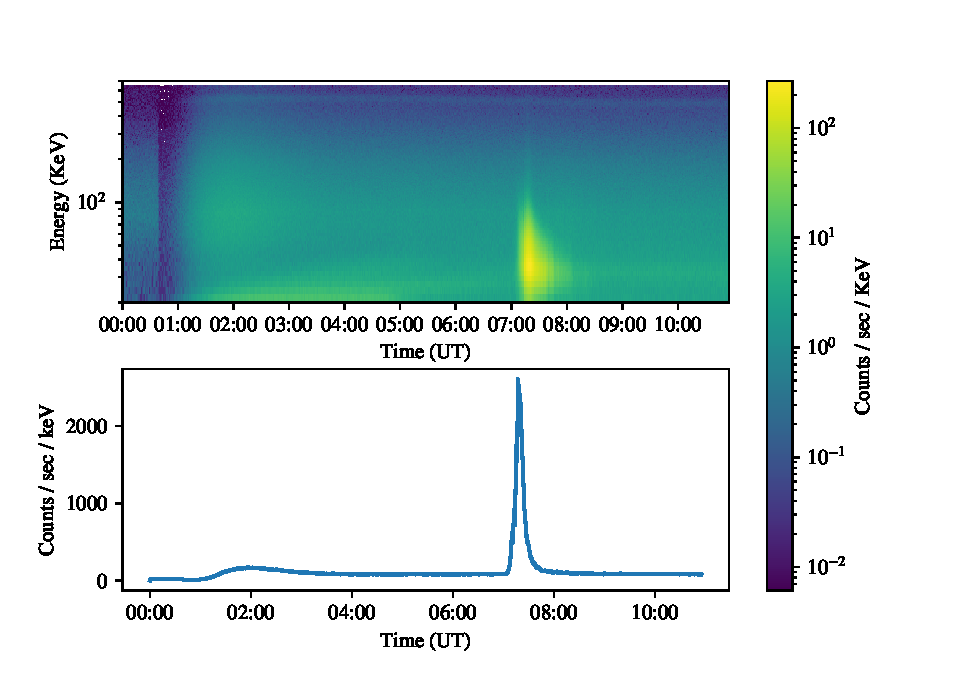
\includegraphics[width=1.0\textwidth]{figures/chapter_5/epex_spectrogram/epex_spectrogram__with_cps_cbar-2}
    \caption{EPEX X-ray spectrometer data in spectrogram form. The precipitation event was observed at 07:00 UTC. The total counts per second are shown below the spectrogram as a function of time.}
    \label{epex_event_spectrogram}
\end{figure}

A background-subtracted spectrum of the precipitation event is shown, along with the reconstruction using the techniques of Chapter 4, in Figure~\ref{epex_fit_comparison}. The retrieved precipitating electron spectrum is shown in Figure~\ref{epex_tk_inv}. The retrieved electron spectrum has a very mono-energetic structure which is centered at approximately 80 keV. The best-fit model agrees well with the data, unlike the result from the $\text{ABOVE}^2$ event, because this detector was flown in a refurbished and undamaged state. The total precipitating electron flux is estimated by the model as $4.8\times 10^8$ electrons $\text{cm}^2$ / second. This was a very bright event which was well-defined in time and energy. The comparatively low value of $\alpha = 3.5\times10^3$ suggested by cross-validation indicates that a good fit to the data was found by the reconstruction algorithms without requiring intense reconditioning of the problem. This is consistent with the fact that this bright event has a very high signal to noise ratio in the background subtracted data. This event can serve as an example of the usefulness of the regularization techniques in analyzing X-ray data. A mono-energetic fit would have certainly been found through application of the forward model, and it could be argued that an exponential fit would be a worse choice based on the $\chi ^2$ statistic. The strength of the regularization methods, combined with cross-validation, is that, with mild assumptions, we can a model-independent characteristic energy and width of the electron distribution. 

\begin{figure}[p]
    \centering
    \includegraphics[width=1.0\textwidth]{figures/chapter_5/epex_fit_comparison/epex_fit_comparison.pdf}
    \caption{Background-subtracted X-ray event measured by the EPEX spectrometer. The model fit using Tikhonov regularization is shown overlaid.}
    \label{epex_fit_comparison}
\end{figure}

\begin{figure}[p]
    \centering
    \includegraphics[width=1.0\textwidth]{figures/chapter_5/epex_tk_inv/epex_tk_inv.pdf}
    \caption{Precipitating electron spectrum retrieved from EPEX X-ray data using the techniques of Chapter 4. The required value for $\alpha$ is low and well-defined through cross-validation.}
    \label{epex_tk_inv}
\end{figure}

\section{The BARREL Campaign}

The BARREL campaign occurred over Antarctica during the year of 2013-2014. There were many flights launched during this campaign and it is beyond the scope of this thesis to analyze all of them using the techniques developed in Chapter~4. There is, however, one flight which stands out as having a high potential new information to be found. ~\citet{Halford2015} examined data from a BARREL balloon which occurred during the aftermath of an ICME (interplanetary coronal mass ejection) shock. The BARREL balloon was airborne and recording data while one of the two RBSP (radiation belt storm probe) spacecraft was on the same approximate L-shell as the balloon. This allowed~\citet{Halford2015} to complete an ``end-to-end'' study of the recorded precipitation event, from creation, to detection by an RBSP spacecraft, to the precipitation in the atmosphere and resulting creation of X-ray radiation detected by the balloon. We will analyze the event measured by the balloon in this chapter, and then consider it in the context of the analysis done by~\citet{Halford2015} in the following chapter. 

A spectrogram of the event observed by~\citet{Halford2015} is shown in Figure~\ref{barrel_spectrogram}. This is a very low intensity event, but it occurs over a long enough time period that the integrated spectrum has a fairly low noise level. The background-subtracted spectrum of the event, and the best-fit model spectrum is shown in Figure~\ref{barrel_fit_comparison.}. Finally, the retrieved electron spectrum is shown in Figure~\ref{barrel_tk_inv}. The retrieved electron spectrum has two main components, a low and fuzzy distribution at around 250 keV, and a smaller high energy component at around 600 to 700 keV. 

\begin{figure}[h]
    \centering
    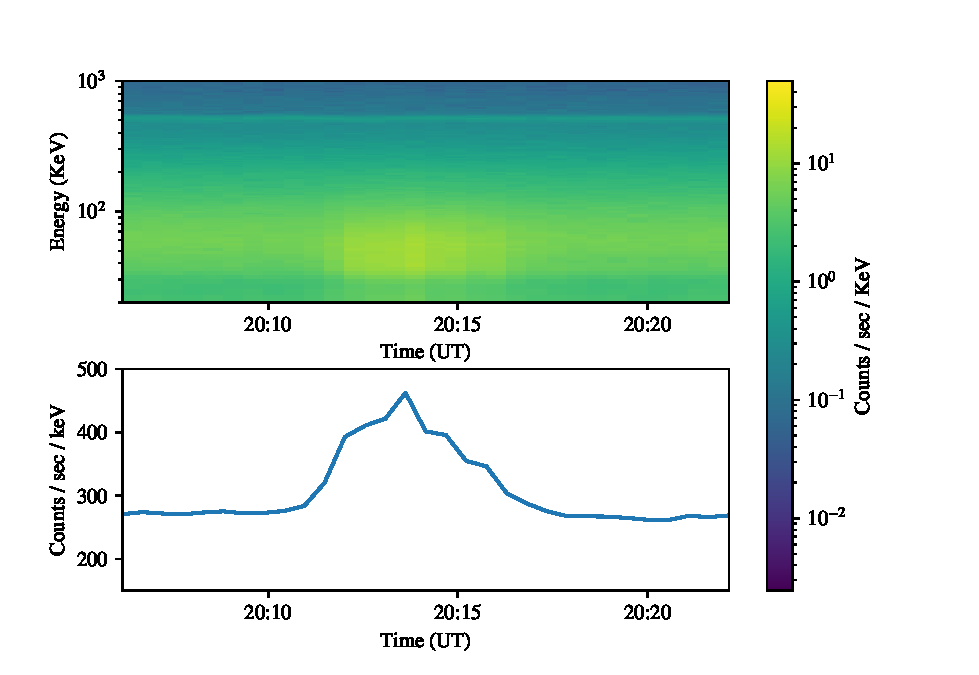
\includegraphics[width=1.0\textwidth]{figures/chapter_5/barrel_spectrogram/barrel_spectrogram}
    \caption{Spectrogram and raw count rates of the event measured by BARREL and studied by~\citet{Halford2015}.}
    \label{barrel_spectrogram}
\end{figure}

\begin{figure}[h]
    \centering
    \includegraphics[width=1.0\textwidth]{figures/chapter_5/barrel_fit_comparison/barrel_fit_comparison}
    \caption{Background-subtracted X-ray event measured by the BARREL spectrometer. The model fit using Tikhonov regularization is shown overlaid.}
    \label{barrel_fit_comparison}
\end{figure}

\begin{figure}[h]
    \centering
    \includegraphics[width=1.0\textwidth]{figures/chapter_5/barrel_tk_inv/barrel_tk_inv}
    \caption{Precipitating electron spectrum retrieved from BARREL X-ray data using the tfechniques of Chapter 4. The required value for $\alpha$ is approximately $5\times10^2$.}
    \label{barrel_tk_inv}
\end{figure}

\section{Inference of Moments and Energy Selective Scattering}

Spacecraft measurements of energetic electrons do not generally resolve the population within the loss cone. The analysis of these data require assumptions about the energy range over which the scattering processes at play operate. We use a published comparison between spacecraft measurements of energetic electrons and their subsequent detection by a BARREL balloon to show that the regularization method developed in Chapter 4 can estimate this energy range. The comparison, published by ~\citet{Halford2015}, uses data from the NASA Radiation Belt Storm Probe (RBSP) spacecraft MAGEIS (magnetic electron ion spectrometer) instruments to make a measurement of the electron population prior to scattering and precipitation to a magnetically proximate BARREL balloon. \citet{Halford2015} uses the relative timing of the two complimentary observations to infer that the precipitating population observed by the balloon was subset to the population observed by the satellite.

Figure~\ref{MAGEIS_measurement} reproduces the spacecraft-measured electron energy spectrum from~\citet{Halford2015}.



